\subsection{Energy Harvesting}
The Screen should be self-sufficient, thus some sort of Energy-Harvesting unit is needed.
It was apparent to choose light as the energy source, since the screen will be used in rooms, which are most of the day artificially illuminated.
A power management chip converts the energy  obtained by solar cells to a suitable voltage.
This way, a super-capacitor, which is used as an energy storage device is charged.

\subsubsection{Solar cell}
The AM-1522 by Panasonic was chosen as the solar cell.
One panel has a area of 55.0 mm $\times$ 40.5 mm and delivers up to 58.7 $\mu\text{A}$ when operating at an optimal voltage of 2.1V, provided an Illumination of 200 lux.
To keep a reasonable display to panel ratio, four cells where used in parallel, which corresponds to an area of ca. 89.1 cm$^2$ (Display area = 283 cm$^2$). Therefore, the solar cells should provide a power of

\begin{align}
	P = U\cdot I = 4\cdot 57.8\ \mu\text{A}\cdot 2.1\ \text{V}=485.52\ \mu \text{W},\label{development:cell_power}
\end{align}

given a 200 lux illumination. \cite{amorton}

\subsubsection{Power management}
The ADP5090 from Analog Devices was used in the power management.
This boost regulator makes it possible to charge storage elements, such as rechargeable batteries and super capacitors with the input dc-power provided by the PV-cell.

Utilized features are:
\begin{itemize}
	\item[-] Maximum power point tracking
	\item[-] Efficiency up to 90\%
	\item[-] Input voltage $V_{in}$ from 80 mV to 3.3 V
	\item[-] Programmable voltage range (2.2 V to 5.2 V) for the storage element
\end{itemize}

To prevent the storage element from overdischarging, the ADP5090 enables the user to set a maximal Voltage with resistors:

\begin{align}
	V_{BAT\_TERM} = \frac{3}{2}\cdot V_{REF}\cdot\left(1+\frac{R_{TERM1}}{R_{TERM2}} \right).\label{development:v_bat_term} 
\end{align} 

The same procedure is applied to set a minimal Voltage:

\begin{align}
	V_{BAT\_SD}=V_{REF}\cdot \left(1+\frac{R_{SD1}}{R_{SD2}} \right).\label{development:v_bat_sd} 
\end{align}  

While discharging, the ADP5090 will switch off the output $V_{SYS}$ if $V_{BAT\_SD}$ is reached. This prevents the storage element from overdischarging.
The output voltage $V_{SYS}$, where the load is attached, will therefore always stay in this programmed range $(V_{BAT\_SD}\le V_{SYS}\le V_{BAT\_TERM})$.
\cite{adp}

\subsubsection{Super capacitor}
As energy Storage, a super capacitor from Taiyo Yuden has proven to be suitable.
The LIC1235RS3R8406 is a 40 F cylinder type lithium ion capacitor.
It's operating voltage range is between 2.2 V and 3.8 V.
Discharging the capacitor lower than 2.2 V causes shorter lifetime and higher leakage.
the same applies to charging the capacitor over 3.8 V.
\cites{yuden}

\subsubsection{Combined test}
To test the behaviour of the power management, supercapacitor and solar cells, a couple of measurements were executed.
The input voltage from the solar cells ($V_in$), voltage of the supercap ($V_{BAT}$) and the output voltage ($V_{SYS}$) were tracked. Additionally, the illuminance near the PV-cells ($E_v$) was recorded.

To carry out the measurement, it was first necessary, to adjust the minimal and maximal voltage of the ADP5090.

\begin{figure}[h]
	\centering
	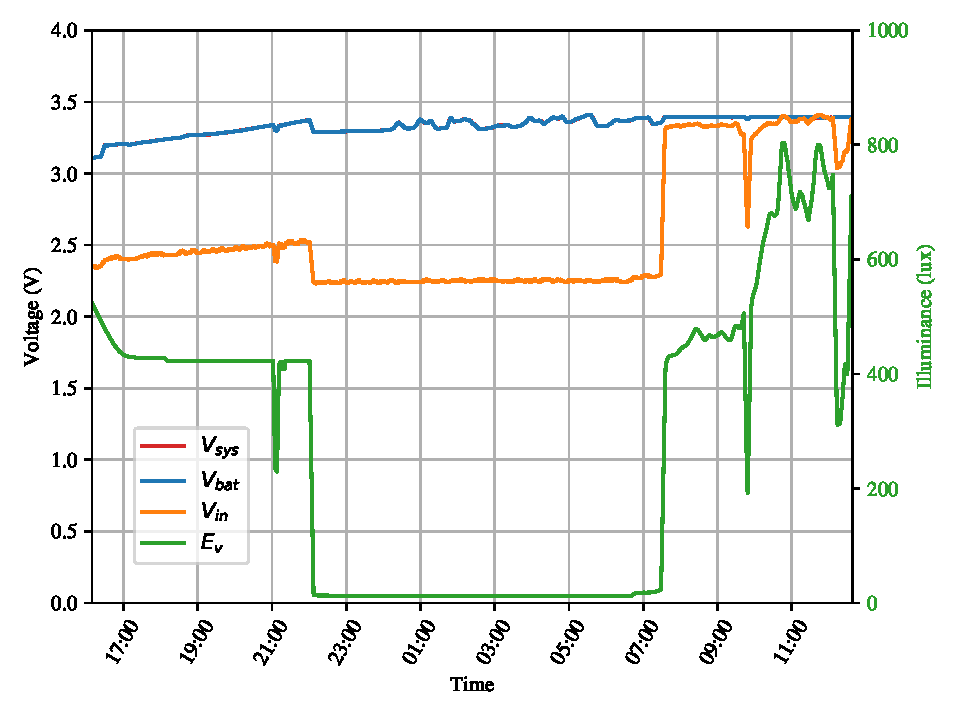
\includegraphics[width=0.9\textwidth]{5-development/hardware/graphics/laden.pdf}
	\caption{Charging behaviour\label{development:charge}}
\end{figure}

\begin{figure}[h]
	\centering
	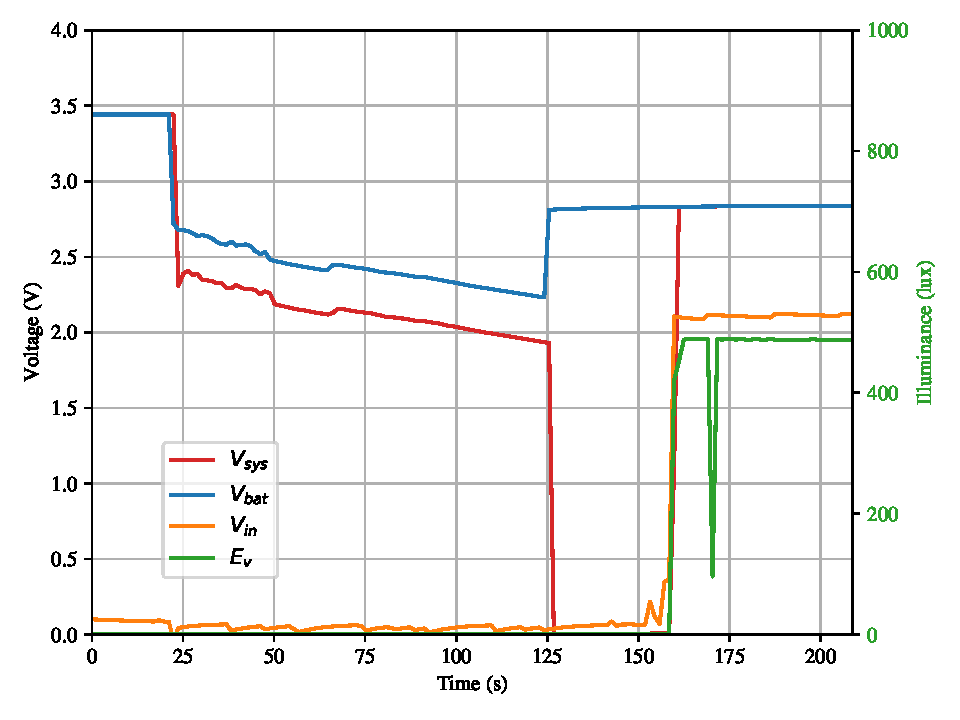
\includegraphics[width=0.9\textwidth]{5-development/hardware/graphics/entladen.pdf}
	\caption{Discharging behaviour\label{development:discharge}}
\end{figure}